\documentclass{beamer}
\hypersetup{pdfpagemode=FullScreen}

%------------------------------------------------------------
% Encoding / language
\usepackage[utf8]{inputenc}
\usepackage[english]{babel}

%------------------------------------------------------------
% Packages
\usepackage{cite}
\usepackage{amsmath,amssymb,amsfonts}
\usepackage{physics}
\usepackage{graphicx}
\usepackage{textcomp}
\usepackage{xcolor}
\usepackage{booktabs}
\usepackage{multirow}
\usepackage{algorithm}
\usepackage{algpseudocode}
\usepackage{comment}
\usepackage{threeparttable}
\usepackage{tikz}
\usepackage{hyperref}
\usepackage[caption=false,font=normalsize,labelfont=sf,textfont=sf]{subfig}
\usepackage{caption}
\captionsetup{labelformat=empty}
\usetikzlibrary{arrows.meta, positioning}

%------------------------------------------------------------
% Theme
\usetheme{Madrid}
\usecolortheme{default}
\setbeamertemplate{navigation symbols}{}

%------------------------------------------------------------
% Custom commands
\newcommand{\presenterbox}[1]{%
\begin{tikzpicture}[remember picture,overlay]
    \node[anchor=south east, xshift=-0.0cm, yshift=0.3cm] at (current page.south east) {%
        \tikz{\node[fill=blue!80, rounded corners=3pt, inner sep=3pt]{\color{white}\small\bfseries #1};}%
    };
\end{tikzpicture}%
}

\captionsetup{
    font=small,
}

%------------------------------------------------------------
% Title page information
\title[RL for Quantum Control]
{Reinforcement-Learning Framework for Robust and Universal Analog Quantum Control on Superconducting Qubits}

\author[F. G. Minisini]
{
    Francesco Giuseppe Minisini\inst{1}\inst{2}
}

\institute[University of Milan / Oslo]
{
      \inst{1} University of Milan
      \and
      \inst{2} University of Oslo
}

\date{Academic Year 2025/2026}

%------------------------------------------------------------
\begin{document}

%------------------------------------------------------------
% Title slide
\begin{frame}
    \titlepage
\end{frame}

%============================================================
\section{Motivation}

\begin{frame}{Why this problem matters}
\begin{columns}[c,onlytextwidth]
    \column{0.52\textwidth}
    \small 

    % \vspace{0.4em}
    \begin{block}{Main difficulty}
    In superconducting qubits, gate design is not only a matter of logical accuracy. Fast pulse-level control must balance several competing goals:
    \end{block}

    \begin{itemize}
        \item \textbf{high gate fidelity}
        \item \textbf{short runtime}
        \item \textbf{low leakage} outside the computational subspace
        \item \textbf{robustness} against control noise
    \end{itemize}

    \column{0.46\textwidth}
    \centering
    \vspace{1.5em}
    \IfFileExists{images/weakly_anharmonic_ladder.pdf}{
        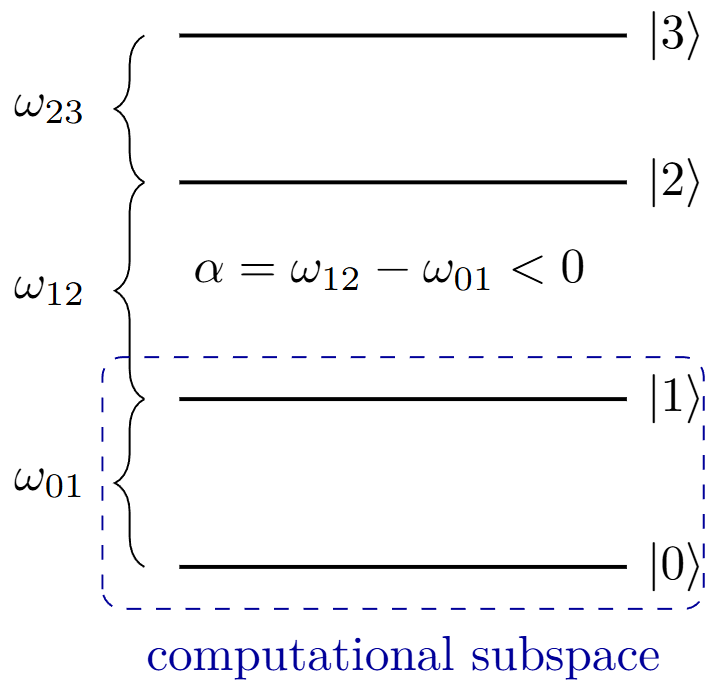
\includegraphics[width=\linewidth, height=0.5\textheight]{images/weakly_anharmonic_ladder.png}
    }{
        \fbox{
            \parbox[c][0.62\textheight][c]{0.92\linewidth}{
                \centering
                Suggested figure:\\[0.3em]
                \texttt{paper\_subspace\_structure.pdf}
            }
        }
    }
\end{columns}

\vspace{0.8em}
\begin{alertblock}{Physical issue}
Superconducting qubits are only \textbf{weakly anharmonic}, so fast control can easily excite unwanted higher levels.
\end{alertblock}

% \presenterbox{Francesco G. Minisini}
\end{frame}

%------------------------------------------------------------
\begin{frame}{Thesis goals and main contribution}
\begin{columns}[T,onlytextwidth]
    \column{0.48\textwidth}
    \small
    \begin{block}{Scientific goal}
    To assess whether the framework proposed by Niu \emph{et al.} is a credible strategy for
    \textbf{robust analog quantum control}.
    \end{block}

    \vspace{0.4em}
    \begin{block}{What I specifically did}
    \begin{itemize}
        \item reconstructed the full framework from the paper
        \item implemented simulation, leakage estimation, and RL pipeline
        \item performed an independent empirical validation
        \item compared nominal, noisy, and family-wide behavior
    \end{itemize}
    \end{block}


    \column{0.48\textwidth}
    \small
    \begin{alertblock}{Important point}
    This was not a standard reproduction from an existing codebase.
    
    \vspace{0.5em}
    \begin{itemize}
        \item No public implementation was available, the whole framework had to be rebuilt from scratch. This included:
        \begin{itemize}
            \item multilevel quantum simulation
            \item TSWT-based leakage estimator
            \item TRPO training pipeline
            \item robustness and runtime experiments
        \end{itemize}
    \end{itemize}
    \end{alertblock}
\end{columns}

% \presenterbox{Francesco G. Minisini}
\end{frame}

%============================================================
\section{Framework}

\begin{frame}{Physical model: gmon Hamiltonian and control channels}
\small
The effective bosonic Hamiltonian is
\vspace{-1ex}
{\scriptsize
\[
\begin{aligned}
    \hat{H}_{\mathrm{RWA}}(t) &=
    \underbrace{\frac{\eta}{2}\sum_{j=1}^{2}\hat{n}_{j}(\hat{n}_{j}-1)}_{\text{anharmonicity}}
    + \underbrace{g(t)(\hat{a}_{2}^{\dagger}\hat{a}_{1}+\hat{a}_{1}^{\dagger}\hat{a}_{2})}_{\text{tunable coupling}} \\
    &\quad + \underbrace{\sum_{j=1}^{2}\delta_{j}(t)\hat{n}_{j}}_{\text{local detuning}}
    + \underbrace{\sum_{j=1}^{2} i f_{j}(t)
    \left(
    \hat{a}_{j}e^{i\phi_{j}(t)}-\hat{a}_{j}^{\dagger}e^{-i\phi_{j}(t)}
    \right)}_{\text{microwave drive}}.
\end{aligned}
\]}
\vspace{-1ex}

% \vspace{-0.2em}
The control vector is:
\(
u(t)=
\bigl(
g(t),\,
\delta_1(t),\delta_2(t),\,
f_1(t),f_2(t),\,
\phi_1(t),\phi_2(t)
\bigr).
\)

% \vspace{0.2em}
% After three-level truncation:
% \[
% d_{\mathrm{phys}}=3^2=9,
% \qquad
% d_{\mathrm{comp}}=4.
% \]

% \vspace{-1em}
\begin{columns}[T,onlytextwidth]
    \column{0.48\textwidth}
    \begin{block}{Meaning of the controls}
    \begin{itemize}
        \item \(g(t)\): tunable inter-qubit coupling
        \item \(\delta_j(t)\): local detunings
        \item \(f_j(t)\): microwave amplitudes
        \item \(\phi_j(t)\): microwave phases
    \end{itemize}
    \end{block}


    \column{0.48\textwidth}
    \begin{alertblock}{Why this matters}
    This is a \textbf{continuous 7-dimensional control problem} on a multilevel superconducting system of dimentionality after three-level truncation: {\scriptsize \(
d_{\mathrm{phys}}=3^2=9,
d_{\mathrm{comp}}=4
\) }
    \end{alertblock}
\end{columns}

% \presenterbox{Francesco G. Minisini}
\end{frame}

%------------------------------------------------------------
\begin{frame}{Why this is a multi-objective control problem}
\small

\begin{block}{UFO objective}
\[
C=
\underbrace{\chi\!\left[1-F(U(T))\right]}_{\text{fidelity penalty}}
+\underbrace{\beta\,L_{\mathrm{tot}}(T)}_{\text{leakage penalty}}
+\underbrace{\mu\,P_{\mathrm{bdry}}}_{\text{boundary penalty}}
+\underbrace{\kappa\,T}_{\text{time penalty}}
\]
\end{block}

\vspace{0.2em}

\scriptsize
\[
F(U(T))=\frac{1}{16}\left|\mathrm{Tr}\!\left(U^\dagger(T)\,U_{\mathrm{target}}\right)\right|^2,
\qquad
P_{\mathrm{bdry}}=\sum_{t\in\{0,T\}}\!\left[g(t)^2+f_1(t)^2+f_2(t)^2\right]
\]
% where \(f(t)^2=f_1(t)^2+f_2(t)^2\).

% \vspace{0.35em}

% \begin{block}{Why multi-objective?}
\begin{itemize}\itemsep0.2em
    \item A good pulse must be \textbf{accurate}, but also \textbf{fast}, \textbf{regular at the boundaries}, and \textbf{low-leakage}.
    \item These goals are not automatically compatible: reducing one penalty can worsen another.
\end{itemize}
% \end{block}

\vspace{0.2em}

\begin{block}{Leakage term: physics-informed proxy}
\scriptsize
\[
L_{\mathrm{tot}}(T)\lesssim
\frac{\|\hat{H}_{\mathrm{od}}(0)\|}{\Delta(0)}
+
\frac{\|\hat{H}_{\mathrm{od}}(T)\|}{\Delta(T)}
+
\int_{0}^{T}
\frac{1}{\Delta(t)^2}
\left\|
\frac{d^2 \hat{H}_{\mathrm{od}}(t)}{dt^2}
\right\|dt
\]
\end{block}

\scriptsize
The first two terms penalize residual couplings at the pulse boundaries; the integral term penalizes rapid temporal variations.

\end{frame}

%------------------------------------------------------------
\begin{frame}{RL formulation}
% \begin{columns}[T,onlytextwidth]
%     \column{0.35\textwidth}
%     % \small
%     % \begin{block}{Target gate family}
%     % \[
%     % N(\alpha,\alpha,\gamma)=
%     % \exp\!\left[
%     % i\left(
%     % \alpha\,\sigma_1^x\sigma_2^x+
%     % \alpha\,\sigma_1^y\sigma_2^y+
%     % \gamma\,\sigma_1^z\sigma_2^z
%     % \right)
%     % \right].
%     % \]
%     % \end{block}

%     % \vspace{0.4em}
%     % This is the family used throughout the numerical study.

%     % \begin{itemize}
%     %     \item continuously parametrized by \(\alpha,\gamma\)
%     %     \item physically meaningful for the gmon interaction structure
%     %     \item suitable for both single-target and family-wide analysis
%     % \end{itemize}

%     % \column{0.48\textwidth}
%     \scriptsize
%     \begin{block}{RL formulation}
%     \begin{itemize}
%         \item \textbf{state}: current propagated unitary \(U_t\)
%         \item \textbf{action}: next continuous control vector
%         \item \textbf{environment}: noisy multilevel quantum dynamics
%         \item \textbf{reward}: negative UFO cost
%         \item \textbf{algorithm}: TRPO actor--critic
%     \end{itemize}
%     \end{block}

%     \column{0.6\textwidth}
    \centering
    % \vspace{1.5em}
    \IfFileExists{images/actor_critic_nn_control.pdf}{
        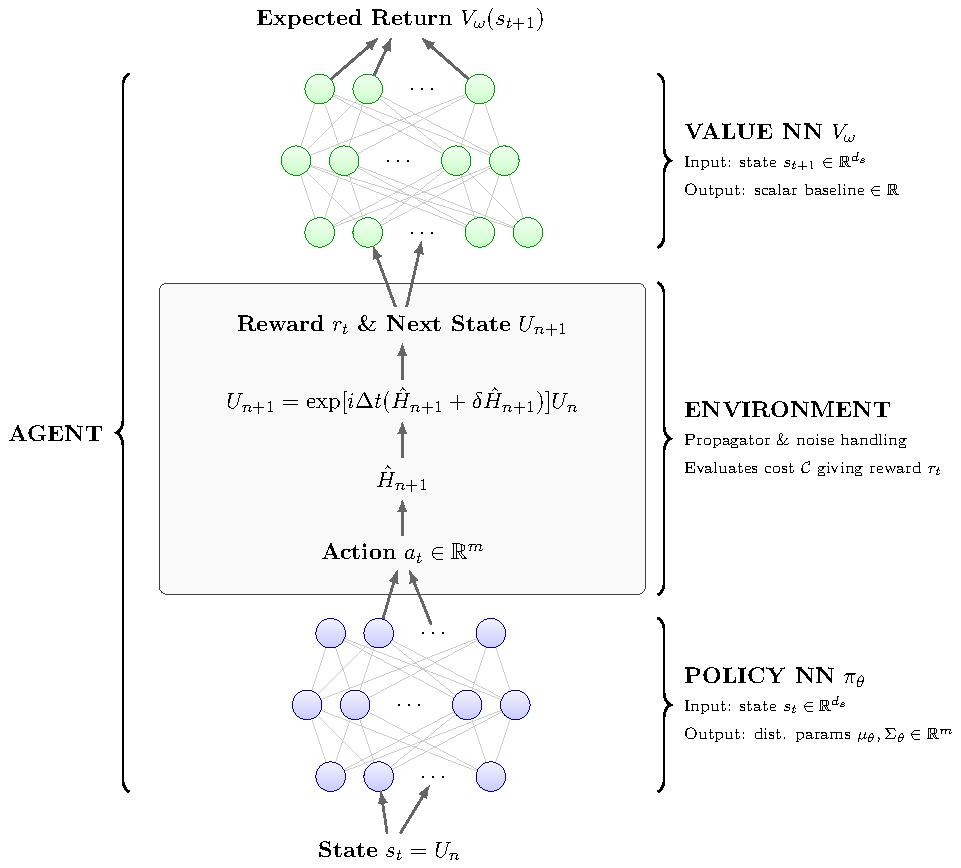
\includegraphics[ height=0.8\textheight]{images/actor_critic_nn_control.pdf}
    }{
        \fbox{
            \parbox[c][0.62\textheight][c]{0.92\linewidth}{
                \centering
                Suggested figure:\\[0.3em]
                \texttt{actor\_critic\_nn\_control.pdf}
            }
        }
    }
% \end{columns}
% \presenterbox{Francesco G. Minisini}
\end{frame}

%------------------------------------------------------------
\begin{frame}{Evaluation metrics \& target gate family}
\scriptsize

%     % \small
\begin{block}{Target gate family used throughout the numerical study.} 
\[
N(\alpha,\alpha,\gamma)=
\exp\!\left[
i\left(
\alpha\,\sigma_1^x\sigma_2^x+
\alpha\,\sigma_1^y\sigma_2^y+
\gamma\,\sigma_1^z\sigma_2^z
\right)
\right].
\]
\end{block}
\vspace{0.4em}

\begin{tabular}{p{0.18\linewidth} p{0.32\linewidth} p{0.42\linewidth}}
\toprule
\textbf{Metric} & \textbf{Definition} & \textbf{Physical meaning} \\
\midrule
Gate fidelity &
\( \scriptstyle
F_{\mathrm{gate}}=
\frac{1}{16}\left|
\mathrm{Tr}\!\left(
U_{\mathrm{proj}}^\dagger(T)U_{\mathrm{target}}
\right)\right|^2
\)
&
Logical accuracy of the implemented two-qubit gate. \\[1em]

Leakage proxy &
\( \scriptstyle
L_{\mathrm{tot}}(T)\lesssim
\frac{\|\hat{H}_{\mathrm{od}}(0)\|}{\Delta(0)}
+
\frac{\|\hat{H}_{\mathrm{od}}(T)\|}{\Delta(T)}
+
\int_{0}^{T}
\frac{1}{\Delta(t)^2}
\left\|
\frac{d^2 \hat{H}_{\mathrm{od}}(t)}{dt^2}
\right\|dt
\)
&
Estimated coherent population loss outside the computational subspace. \\[3em]

Average fidelity under noise &
\( \scriptstyle
\overline{F}(\sigma)=
\mathbb{E}[F]
\)
&
Mean gate performance over many noisy Monte Carlo realizations. \\[1em]

Fidelity variance &
\( \scriptstyle
\mathrm{Var}(F)=\mathbb{E}\big[(F-\overline{F})^2\big]
\)
&
Shot-to-shot stability under stochastic perturbations. \\[1em]
\bottomrule
\end{tabular}

% \vspace{0.4em}
% \small
% \begin{alertblock}{Key point}
% A good controller must be not only accurate, but also fast, low-leakage, and robust.
% \end{alertblock}

% \presenterbox{Francesco G. Minisini}
\end{frame}

%============================================================
\section{Implementation}

% \begin{frame}{Framework reconstruction from scratch}
% \begin{columns}[T,onlytextwidth]
%     \column{0.52\textwidth}
%     \small
%     \begin{block}{What had to be implemented}
%     \begin{itemize}
%         \item multilevel gmon simulator
%         \item bandwidth-limited control filtering
%         \item TSWT-based leakage estimator
%         \item RL environment and TRPO agent
%         \item training, evaluation, and robustness pipelines
%         \item runtime sweeps across the gate family
%     \end{itemize}
%     \end{block}

%     \vspace{0.4em}
%     \begin{alertblock}{Why this is relevant}
%     The thesis contribution is not only empirical testing:
%     it includes the \textbf{full reconstruction} of a nontrivial hybrid framework joining
%     quantum simulation, leakage physics, and reinforcement learning.
%     \end{alertblock}

%     \column{0.48\textwidth}
%     \centering
%     \IfFileExists{figures/framework_overview.png}{
%         \includegraphics[width=\linewidth]{figures/framework_overview.png}
%     }{
%         \IfFileExists{chapters/plots/paper_rl_loop.pdf}{
%             
\includegraphics[width=\linewidth]{chapters/plots/paper_rl_loop.pdf}
%         }{
%             \fbox{
%                 \parbox[c][0.62\textheight][c]{0.92\linewidth}{
%                     \centering
%                     Put here your framework image\\[0.3em]
%                     (the one you sent me),\\[0.4em]
%                     or fallback to \texttt{paper\_rl\_loop.pdf}
%                 }
%             }
%         }
%     }
% \end{columns}

% % \presenterbox{Francesco G. Minisini}
% \end{frame}

\begin{frame}

    distinzione tra noise optimized e nominal agent
    
    lista di esperimenti runnati e motivazioni
    \begin{itemize}
        \item 
    \end{itemize}
\end{frame}

%------------------------------------------------------------
\begin{frame}{Extended parameter study}
\scriptsize
In RL, parameter choice strongly affects stability, convergence, robustness, and final control quality. I performed an extended study on:

\vspace{0.3em}
\begin{columns}[T,onlytextwidth]
    \column{0.48\textwidth}
    \textbf{Policy/value architectures}
    \begin{itemize}
        \item sweep over 5 network topologies
        \item final choice: \((64,32,32)\)
    \end{itemize}
    
    \vspace{0.4em}
    \centering
    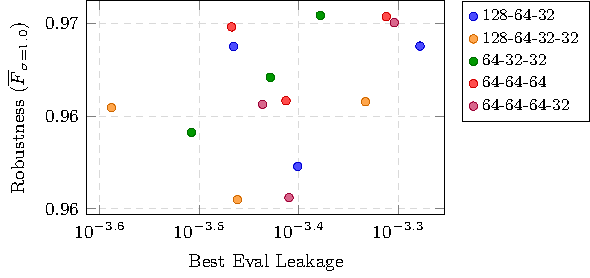
\includegraphics[width=0.95\linewidth, height=0.35\textheight, keepaspectratio]{images/architecture_sweep_pareto.pdf}

    \column{0.48\textwidth}
    \textbf{UFO weights}
    \begin{itemize}
        \item sensitivity study over 36 configurations
        \item final choice: \((10,10,0.2,0.1)\)
    \end{itemize}

    \vspace{-0.4em}
    \centering
    
\includegraphics[width=\linewidth, height=0.33\textheight, keepaspectratio]{images/ufo_weight_sweep_pareto.pdf}
\end{columns}

\vspace{0.5em}
\centering

\includegraphics[width=0.95\linewidth, height=0.25\textheight, keepaspectratio]{images/ufo_weight_sweep_robustness.pdf}

\end{frame}

%============================================================
\section{Results}

\begin{frame}{Single-target optimization: Dynamics and Horizon}
\small
Representative target: \(N(2.2,2.2,\pi/2)\). We analyze the TRPO training evolution and the Adam runtime horizon.

\vspace{0.5em}
\begin{columns}[c,onlytextwidth]
    \column{0.48\textwidth}
    \centering
    \textbf{TRPO training dynamics}\\
    \vspace{0.2em}
    
\includegraphics[width=0.95\linewidth, height=0.6\textheight, keepaspectratio]{images/nominal_trpo_training_curves.pdf}
    
    \column{0.48\textwidth}
    \centering
    \textbf{Single-target horizon sweep}\\
    \vspace{0.2em}
    
\includegraphics[width=0.95\linewidth, height=0.6\textheight, keepaspectratio]{images/adam_single_target_horizon_sweep.pdf}
\end{columns}

    \centering
    \footnotesize
    \begin{tabular}{lcccc}
    \toprule
    \textbf{Method} & \textbf{Time (ns)} & \textbf{Cost} & \textbf{Fidelity} & \textbf{Leakage} \\
    \midrule
    Adam & 70 & 0.157 & 0.9966 & \(2.8\times 10^{-4}\) \\
    TRPO & 116 & 0.298 & 0.9941 & \(1.6\times 10^{-3}\) \\
    \bottomrule
    \end{tabular}

\end{frame}

%------------------------------------------------------------
\begin{frame}{Adam vs TRPO and Family-wide evaluation}

% \begin{block}{Single-target: Adam vs TRPO performance}
    \centering
    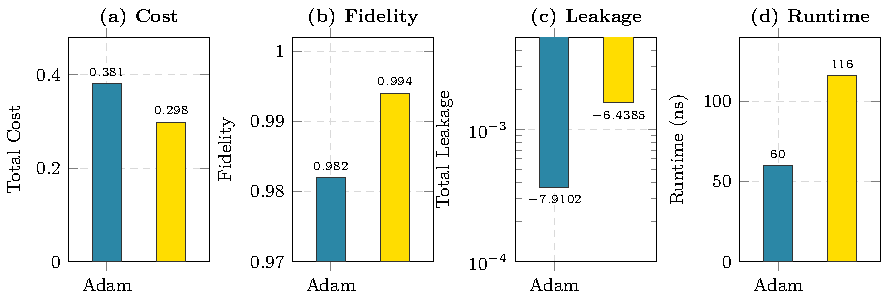
\includegraphics[width=\linewidth, height=0.3\textheight, keepaspectratio]{images/single_target_adam_vs_nominal_trpo.pdf}
    
% \end{block}

% \begin{block}{Family-wide runtime sweep}
\small
Family-wide runtime sweep was also evaluated to mostly assess performance consistency across the target gate family of the Adam baseline.

\vspace{0.1em}
\centering
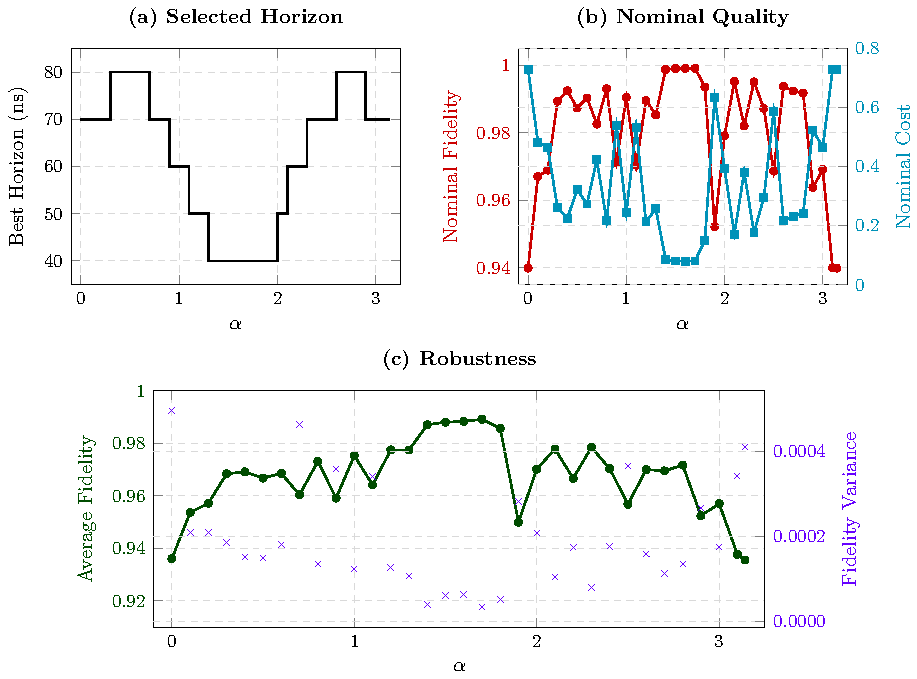
\includegraphics[ height=0.5\textheight, keepaspectratio]{images/adam_family_sweep.pdf}
% \end{block}
\end{frame}

%------------------------------------------------------------
% \begin{frame}{Noise-optimized TRPO: representative training dynamics}
% \begin{columns}[T,onlytextwidth]
%     \column{0.42\textwidth}
%     \small
%     \begin{block}{What this plot shows}
%     A representative training run of the learned controller:
%     \end{block}

%     \begin{itemize}
%         \item evaluation cost
%         \item execution time
%         \item fidelity
%         \item leakage
%     \end{itemize}

%     \vspace{0.4em}
%     \begin{alertblock}{Interpretation}
%     Training is not monotonic: the policy must learn how to balance
%     fidelity, leakage, and runtime at the same time.
%     \end{alertblock}

%     \vspace{0.3em}
%     Sharp spikes typically correspond to runs that fail to terminate early and saturate the time bound.

%     \column{0.58\textwidth}
%     \centering
%     \IfFileExists{chapters/plots/noise_optimized_trpo_training_curves.pdf}{
%         \includegraphics[width=\linewidth]{chapters/plots/noise_optimized_trpo_training_curves.pdf}
%     }{
%         \IfFileExists{chapters/plots/nominal_trpo_training_curves.pdf}{
%             
\includegraphics[width=\linewidth]{chapters/plots/nominal_trpo_training_curves.pdf}
%         }{
%             \fbox{
%                 \parbox[c][0.62\textheight][c]{0.92\linewidth}{
%                     \centering
%                     Put here the training-curves figure of the\\
%                     noise-optimized run.\\[0.4em]
%                     Current fallback:\\
%                     \texttt{nominal\_trpo\_training\_curves.pdf}
%                 }
%             }
%         }
%     }
% \end{columns}

% % \presenterbox{Francesco G. Minisini}
% \end{frame}

%------------------------------------------------------------
\begin{frame}{Noise-optimized Agent: Robustness}
\small
Under Gaussian control noise, the \textbf{noise-optimized TRPO controller} becomes the strongest overall method. The key advantage is not just RL itself, but \textbf{RL trained in the correct stochastic environment}.

\vspace{0.3em}
\begin{columns}[T,onlytextwidth]
    \column{0.48\textwidth}
    \textbf{Average fidelity}
    \begin{itemize}
        \item retains highest \(\overline{F}(\sigma_{\mathrm{noise}})\)
        \item outperforms Adam and nominal TRPO
    \end{itemize}
    
    \vspace{0.2em}
    \centering
    
\includegraphics[width=0.95\linewidth, height=0.55\textheight, keepaspectratio]{images/avg_fidelity_vs_noise.pdf}
    
    \column{0.48\textwidth}
    \textbf{Fidelity variance}
    \begin{itemize}
        \item demonstrates lowest \(\mathrm{Var}(F)\)
        \item superior structural stability under noise
    \end{itemize}
    
    \vspace{0.2em}
    \centering
    
\includegraphics[width=0.95\linewidth, height=0.55\textheight, keepaspectratio]{images/fidelity_variance_vs_noise.pdf}
\end{columns}
\end{frame}

%------------------------------------------------------------
\begin{frame}{Runtime across the gate family \(N(\alpha,\alpha,\pi/2)\)}
\begin{columns}[T,onlytextwidth]
    \column{0.52\textwidth}
    \small
    \[
    U_{\mathrm{target}}(\alpha)=N(\alpha,\alpha,\pi/2)
    \]

    \vspace{0.4em}
    \begin{itemize}
        \item The runtime landscape is \textbf{highly structured}, not uniform.
        \item A broad central region admits significantly faster analog solutions.
        \item The analog controller stays below the gate-synthesis reference over a large part of the family.
    \end{itemize}

    \vspace{0.4em}
    \begin{block}{Reference benchmark}
    \[
    T_{\mathrm{syn}} \approx 215\,\mathrm{ns}
    \]
    from optimal discrete gate synthesis.
    \end{block}

    \vspace{0.4em}
    \begin{alertblock}{Physical interpretation}
    The strongest speedups appear where the target gate is better aligned with the native hardware interaction.
    \end{alertblock}

    \column{0.48\textwidth}
    \centering
    \IfFileExists{chapters/plots/runtime_vs_alpha.pdf}{
        
\includegraphics[width=\linewidth]{chapters/plots/runtime_vs_alpha.pdf}
    }{
        \fbox{
            \parbox[c][0.62\textheight][c]{0.92\linewidth}{
                \centering
                Suggested figure:\\[0.3em]
                \texttt{runtime\_vs\_alpha.pdf}
            }
        }
    }
\end{columns}

% \presenterbox{Francesco G. Minisini}
\end{frame}

%============================================================
\section{Conclusions}

\begin{frame}{Conclusions}
\small
\begin{columns}[T,onlytextwidth]
    \column{0.52\textwidth}
    \begin{block}{Scientific conclusions}
    \begin{itemize}
        \item The framework is physically meaningful and empirically credible.
        \item In the nominal single-target regime, direct pulse optimization remains very strong.
        \item Under stochastic perturbations, noise-optimized RL becomes the best strategy.
        \item Analog control can outperform standard gate synthesis in runtime.
    \end{itemize}
    \end{block}

    \column{0.48\textwidth}
    \begin{block}{What this thesis contributed}
    \begin{itemize}
        \item full reconstruction of the framework from scratch
        \item implementation of simulation, leakage, and RL pipeline
        \item extended parameter study
        \item independent validation of strengths and limitations
    \end{itemize}
    \end{block}
\end{columns}

\vspace{0.5em}
\begin{alertblock}{Final message}
The main value of this framework is not universal nominal dominance,
but a \textbf{unified strategy for robust, leakage-aware, hardware-relevant analog quantum control}.
\end{alertblock}

% \presenterbox{Francesco G. Minisini}
\end{frame}

%------------------------------------------------------------
\end{document}